\documentclass[crop,tikz]{standalone}% 'crop' is the default for v1.0, before it was 'preview'
\usepackage{tikz}
\usepackage{tikz-3dplot}
\usetikzlibrary{calc}
\usetikzlibrary{decorations.pathmorphing, patterns,shapes,arrows.meta}
\usetikzlibrary{plotmarks}
\usetikzlibrary{matrix}
\usetikzlibrary{external,calc,patterns,decorations.pathmorphing}
\usetikzlibrary{shapes.geometric}
\usetikzlibrary{decorations.markings}
\usepackage{pgfplots}
\usetikzlibrary{backgrounds}
\begin{document}
	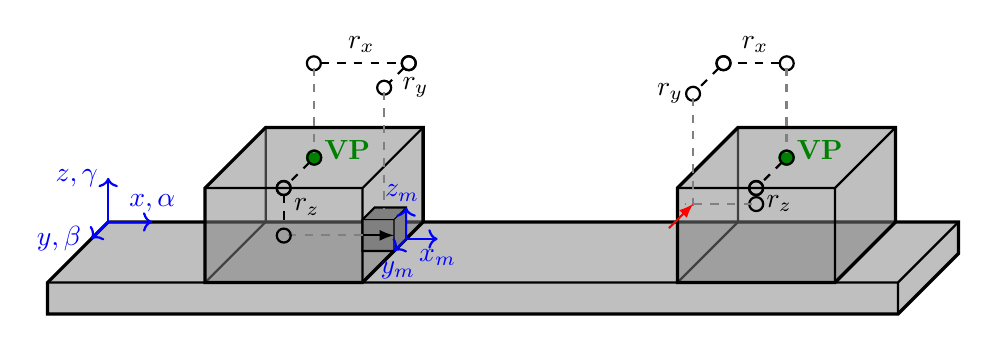
\begin{tikzpicture}
		[scale = 0.8,
		sensor/.style={fill opacity=1,thick,fill=gray,line cap =butt},
        block/.style={fill opacity=.5,very thick,fill=gray,line cap =round},
        clear/.style={fill opacity=.0,very thick,fill=gray,line cap =round},
		hidden/.style={very thick,dashed},
		grid/.style={very thin,gray},
		axis/.style={->,blue,thick},
        cross/.style={path picture={ 
          \draw[black]
            (path picture bounding box.south east) -- (path picture bounding box.north west) (path picture bounding box.south west) -- (path picture bounding box.north east);}}
        ]


        % Main block
	    	    \def \x {-2.5}
        \def \y {-0.5}
        \def \z {0}
        \def \sx {13.5}
        \def \sy {0.5}
        \def \sz {2.5}
        %draw the front-right of the cube
        \draw[block] (\x,\y+\sy,\z) -- (\x+\sx,\y+\sy,\z) -- (\x+\sx,\y,\z) -- (\x+\sx,\y,\z+\sz) -- (\x,\y,\z+\sz) -- (\x,\y+\sy,\z+\sz) -- cycle;
	    \draw[black,thick,line cap=round] (\x+\sx,\y+\sy,\z+\sz) -- (\x,\y+\sy,\z+\sz) (\x+\sx,\y+\sy,\z+\sz) -- (\x+\sx,\y,\z+\sz) (\x+\sx,\y+\sy,\z+\sz) -- (\x+\sx,\y+\sy,\z);

        \def \x {0}
        \def \y {0}
        \def \z {0}
        \def \sx {2.5}
        \def \sy {1.5}
        \def \sz {2.5}
        	\draw[black,thick,line cap=round] (\x,\y,\z+\sz) -- (\x,\y,\z) (\x+\sx,\y,\z) -- (\x,\y,\z) (\x,\y,\z) -- (\x,\y+\sy,\z);
	\draw[block] (\x,\y+\sy,\z) -- (\x+\sx,\y+\sy,\z) -- (\x+\sx,\y,\z) -- (\x+\sx,\y,\z+\sz) -- (\x,\y,\z+\sz) -- (\x,\y+\sy,\z+\sz) -- cycle;
	\draw[black,thick,line cap=round] (\x+\sx,\y+\sy,\z+\sz) -- (\x,\y+\sy,\z+\sz) (\x+\sx,\y+\sy,\z+\sz) -- (\x+\sx,\y,\z+\sz) (\x+\sx,\y+\sy,\z+\sz) -- (\x+\sx,\y+\sy,\z);


         % Sensor 7
        \def \x {2.5}
        \def \y {0.5}
        \def \z {2}
        \def \s {0.5}
        %draw the front-right of the cube
        \draw[sensor] (\x,\y+\s,\z) -- (\x+\s,\y+\s,\z) -- (\x+\s,\y,\z) -- (\x+\s,\y,\z+\s) -- (\x,\y,\z+\s) -- (\x,\y+\s,\z+\s) -- cycle;
	\draw[black,line cap=round] (\x+\s,\y+\s,\z+\s) -- (\x,\y+\s,\z+\s) (\x+\s,\y+\s,\z+\s) -- (\x+\s,\y,\z+\s) (\x+\s,\y+\s,\z+\s) -- (\x+\s,\y+\s,\z);
        \draw[black,thick,-latex] (\x,\y+\s/2,\z+\s) -- (\x+\s,\y+\s/2,\z+\s);
        \node[] at (\x-0.35,\y+0.1,\z) {};


        \draw[green!50!black,thick,shorten >=-3pt,shorten <=-3pt,*-*] (1.25,1.5,1.25) -- (1.25,1.5,1.25) node[right,yshift = 0.1cm] {\textbf{VP}};

        \draw[black,dashed,thick,o-o,shorten >=-3pt,shorten <=-3pt] (1.25,3,1.25) -- (2.75,3,1.25) node[pos=0.5,above] {$r_x$};
        \draw[black,dashed,thick,o-o,shorten >=-3pt,shorten <=-3pt] (2.75,3,1.25)  -- (2.75,3,2.25) node[pos=1,right,xshift=0.1cm] {$r_y$};        
        \draw[white!50!black,dashed,thick,shorten >=-3pt,shorten <=-3pt] (1.25,2.8,1.25) -- (1.25,1.7,1.25);
        \draw[white!50!black,dashed,thick,shorten >=-3pt,shorten <=-3pt] (2.75,2.8,2.25) -- (2.75,1.2,2.25);
        \draw[white!50!black,dashed,thick,shorten >=-3pt,shorten <=-3pt] (1.45,0.75,2.5) -- (2.5,0.75,2.5);
        \draw[black,dashed,thick,o-o,shorten >=-3pt,shorten <=-3pt] (1.25,1.5,1.25) -- (1.25,1.5,2.5) node[pos=0,above] {};
        \draw[black,dashed,thick,o-o,shorten >=-3pt,shorten <=-3pt] (1.25,1.5,2.5) -- (1.25,0.75,2.5) node[pos=0.4,right] {$r_z$};



        %draw the axes
	    \draw[axis] (-2.5,0,0) -- +(0.7,0,0) node[anchor=south]{$x,\alpha$};
	    \draw[axis] (-2.5,0,0) -- +(0,0.7,0) node[anchor=east]{$z,\gamma$};
	    \draw[axis] (-2.5,0,0) -- +(0,0,0.7) node[anchor=east]{$y,\beta$};

        %draw the axes
	    \draw[axis] (3,0.5,2) -- +(0.5,0,0) node[anchor=north]{$x_m$};
	    \draw[axis] (3,0.5,2) -- +(0,0.5,0) node[anchor=south,xshift = -0.05cm,yshift = -0.05cm]{$z_m$};
	    \draw[axis] (3,0.5,2) -- +(0,0,0.5) node[anchor=north, xshift=0.05cm]{$y_m$};


        \begin{scope}[transform canvas={xshift = 6cm}]
    
            % Main block
    	    \def \x {0}
            \def \y {0}
            \def \z {0}
            \def \sx {2.5}
            \def \sy {1.5}
            \def \sz {2.5}
            	\draw[black,thick,line cap=round] (\x,\y,\z+\sz) -- (\x,\y,\z) (\x+\sx,\y,\z) -- (\x,\y,\z) (\x,\y,\z) -- (\x,\y+\sy,\z);
	\draw[block] (\x,\y+\sy,\z) -- (\x+\sx,\y+\sy,\z) -- (\x+\sx,\y,\z) -- (\x+\sx,\y,\z+\sz) -- (\x,\y,\z+\sz) -- (\x,\y+\sy,\z+\sz) -- cycle;
	\draw[black,thick,line cap=round] (\x+\sx,\y+\sy,\z+\sz) -- (\x,\y+\sy,\z+\sz) (\x+\sx,\y+\sy,\z+\sz) -- (\x+\sx,\y,\z+\sz) (\x+\sx,\y+\sy,\z+\sz) -- (\x+\sx,\y+\sy,\z);

            \draw[green!50!black,thick,shorten >=-3pt,shorten <=-3pt,*-*] (1.25,1.5,1.25) -- (1.25,1.5,1.25) node[right,yshift = 0.1cm] {\textbf{VP}};

            \draw[black,dashed,thick,o-o,shorten >=-3pt,shorten <=-3pt] (1.25,3,1.25) -- (0.25,3,1.25) node[pos=0.5,above] {$r_x$};
            \draw[black,dashed,thick,o-o,shorten >=-3pt,shorten <=-3pt] (0.25,3,1.25)  -- (0.25,3,2.5) node[pos=1,left,xshift=0cm] {$r_y$};        
            \draw[white!50!black,dashed,thick,shorten >=-3pt,shorten <=-3pt] (1.25,2.8,1.25) -- (1.25,1.7,1.25);
            \draw[white!50!black,dashed,thick,shorten >=-3pt,shorten <=-3pt] (0.25,2.8,2.5) -- (0.25,1.3,2.5);
            \draw[red,thick,-latex] (0.25,1.25,3.5) -- (0.25,1.25,2.5) node[pos=0,anchor=north east] {};

            \draw[black,dashed,thick,o-o,shorten >=-3pt,shorten <=-3pt] (1.25,1.5,1.25) -- (1.25,1.5,2.5) node[pos=0,above] {};
            \draw[black,dashed,thick,o-o,shorten >=-3pt,shorten <=-3pt] (1.25,1.5,2.5) -- (1.25,1.25,2.5) node[pos=1,right,xshift=-0.cm] {$r_z$};     \draw[white!50!black,dashed,thick,shorten >=-3pt,shorten <=-3pt] (1.05,1.25,2.5) -- (0.25,1.25,2.5);

        \end{scope}
\end{tikzpicture}
\end{document}